\documentclass[Afour,sageh,times]{sagej}
\usepackage{moreverb,url}

\usepackage[colorlinks,bookmarksopen,bookmarksnumbered,citecolor=red,urlcolor=red]{hyperref}

\usepackage{chngpage}

\newcommand\BibTeX{{\rmfamily B\kern-.05em \textsc{i\kern-.025em b}\kern-.08em
T\kern-.1667em\lower.7ex\hbox{E}\kern-.125emX}}

\def\volumeyear{2017}


\usepackage[utf8]{inputenc}
\usepackage[T1]{fontenc}

%%%%%
% variable to include comments or not in the compilation ; set to 1 to include
%\def \draft {1}
\def \draft {0}



\usepackage{xparse}
\usepackage{ifthen}

\DeclareDocumentCommand{\comment}{o m o o o o}
{\ifthenelse{\draft=1}{
  \IfValueT{#1}{
      \textcolor{red}{\textbf{C (#1) : }#2}
      \IfValueT{#3}{\textcolor{blue}{\textbf{A1 : }#3}}
      \IfValueT{#4}{\textcolor{ForestGreen}{\textbf{A2 : }#4}}
      \IfValueT{#5}{\textcolor{red!50!blue}{\textbf{A3 : }#5}}
      \IfValueT{#6}{\textcolor{Aquamarine}{\textbf{A4 : }#6}}
    }
    \IfNoValueT{#1}{
      \textcolor{red}{\textbf{C : }#2}
      \IfValueT{#3}{\textcolor{blue}{\textbf{A1 : }#3}}
      \IfValueT{#4}{\textcolor{ForestGreen}{\textbf{A2 : }#4}}
      \IfValueT{#5}{\textcolor{red!50!blue}{\textbf{A3 : }#5}}
      \IfValueT{#6}{\textcolor{Aquamarine}{\textbf{A4 : }#6}}
    }
 }{}
}




% todo
%\newcommand{\todo}[1]{
%\ifthenelse{\draft=1}{\textcolor{red!50!blue}{\textbf{TODO : \textit{#1}}}}{}
%}
\DeclareDocumentCommand{\todo}{o m}{
  \ifthenelse{\draft=1}{
    \IfValueT{#1}{\textcolor{red!50!blue}{\textbf{TODO (#1) : \textit{#2}}}}
    \IfNoValueT{#1}{\textcolor{red!50!blue}{\textbf{TODO : \textit{#2}}}}
  }{}
}

%\date{}
%\renewcommand\abstractname{\fontsize{14pt}{0}\textbf{Abstract}\selectfont}

%\usepackage[left=25mm, right=25mm, top=25mm, bottom=25mm, includehead=false, includefoot=false]{geometry}

%\usepackage{graphicx}
%\usepackage{url}
%\usepackage[round,semicolon]{natbib}  % Citation styles https://www.sharelatex.com/learn/Natbib_citation_styles
%\bibliographystyle{humannat}
%\renewcommand{\bibsection}{}
%\renewcommand{\bibhang}{\setlength{-1px}}


%\usepackage{authblk} % For author lists
%\renewcommand\Authfont{\fontsize{11}{1}\selectfont}
%\renewcommand\Affilfont{\fontsize{9}{1}\selectfont}

%\renewcommand*\footnoterule{}

\usepackage[table]{xcolor}
\usepackage[parfill]{parskip} % Line between paragraphs
\usepackage{amsmath}
%\pagenumbering{arabic} 

%\usepackage{sectsty}
%\allsectionsfont{\sffamily}

%\usepackage[pdftex]{hyperref} 
%\hypersetup{pdfborder={0 0 0} }


\usepackage[flushleft]{threeparttable}



%%%%%%%%%%%%%%%%%%%%%%%%%
%% -- from ecrc template
%%%%%%%%%%%%%%%%%%%%%%%%%


%% set the volume if you know. Otherwise `00'
\volume{00}

%% set the starting page if not 1
\firstpage{1}



\jid{}


\biboptions{authoryear}




\usepackage{soul}
\soulregister\cite7
\soulregister\citep7
\soulregister\ref7

%\usepackage[final]{changes}
\usepackage{changes}


\setaddedmarkup{\textcolor{black}{\hl{#1}}}
\setdeletedmarkup{\textcolor{red}{\sout{#1}}}

% add line number
\usepackage{lineno}
\linenumbers








\begin{document}

% **************  TITLE AND AUTHOR INFORMATION **************


\runninghead{Raimbault \& al.}


\title{Initial spatial conditions in simulation models: the missing leg of sensitivity analyses?}

\author{Juste Raimbault\affilnum{1,2}, 
Cl{\' e}mentine Cottineau\affilnum{3},
Marion Le Texier\affilnum{4}, 
Florent Le N{\' e}chet\affilnum{2}, 
Romain Reuillon\affilnum{1,5}
}

\affiliation{\affilnum{1}UMR 8504 G{\'e}ographie-cit{\'e}s, Paris, France\\
\affilnum{2}Laboratoire Ville Mobilit{\'e} Transport, Universit{\'e} Paris-Est, France\\
\affilnum{3}Centre for Advanced Spatial Analysis, University College London, UK\\
\affilnum{4}UMR 6266 IDEES, Universit{\'e} de Rouen Normandie, France\\
\affilnum{5}Institut des Syst{\`e}mes Complexes Paris Ile-de-France, France}

\corrauth{Corresponding author
address.}

\email{c.cottineau@ucl.ac.uk}



% **************  ABSTRACT  **************

\begin{abstract}
%\noindent
%\setlength{\parindent}{0pt}
Although simulation models of geographical systems in general and agent-based models in particular represent a fantastic opportunity to explore socio-spatial behaviours and to test a variety of scenarios for public policy, the validity of generative models is uncertain until their results are proven robust. Sensitivity analysis usually include the analysis of the effect of stochasticity on the variability of results, as well as the effects of small parameter changes. However, initial spatial conditions are usually taken for granted in geographical models, thus leaving completely unexplored the effect of spatial arrangements on the interaction of agents and of their interactions with the environment. In this contribution, we present a method to assess the effect of initial spatial conditions on simulation models, using a systematic generator controlled by meta-parameter to create density grids used in spatial simulation models. We show, with the example of two very classical agent-based models (Schelling's models of segregation and Sugarscape) that the effect of space in simulation is significant, and sometimes even larger than parameters themselves. We do so using high performance computing in a very simple and straightforward open-source workflow.
\end{abstract}

\keywords{Space, Initial conditions, Sensitivity, ABM}

\maketitle


% **************  MAIN BODY OF THE PAPER **************


%%%%%%%%%%%%%%%%%%%%%%
\section{Introduction}
%%%%%%%%%%%%%%%%%%%%%%

Simulation has been recognised and increasingly used by geographers to explore various geographical processes and problems within virtual laboratories \citep{Quesneletal2009} \comment{Batty 1978? James Doran 1970's : lire thèse de Seb ;) }. It appears as a very fruitful way to overcome the difficulty of analytic resolution of many spatial models developed in the past, and to explore the possible trajectories of social and ecological systems in space and time. The specificity of geographical models compared with models from other social sciences is usually regarded as the way geographers consider space and spatial interactions, driven by an explicit interest in the way space influences the outcomes of the model. Geographers are indeed concerned about understanding and modelling how space plays a role in social interactions and environmental processes, and whether its action is placed-based or place-neutral. We think simulation can become a very good tool to achieve this, provided that models include relevant spatial description and modelling, behavioural rules that take space into account, and provided model evaluation stresses the sensitivity of output variations to the way space is modelled. This paper aims to fill a methodological and conceptual gap, which is a systematic testing of the sensitivity of model's outcomes to initial spatial conditions. To demonstrate the genericity of our approach, we develop two applications from simulation models which are commonly used as case studies for comparing and aligning simulation models \citep{Axtelletal1996}: Schelling's model of segregation and Epstein and Axtell's Sugarscape model. Both models are defined at the intraurban level.

\subsection{Objective}

In this paper, we suggest tackling sensitivity to spatial conditions by generating a variety of density grids to feed into simulation models at initialisation, and exploring the sensitivity of the model outcomes to the variation of meta-parameters (i.e. parameters used to generate initial spatial conditions). The purpose is two-fold: 1/ to test the robustness of simulation results to small variations of meta-parameters within a typical category of space (a monocentric case for example) and 2/ to study the non-trivial effects of typical categories of spatial distribution (monocentric vs. polycentric for example) on the results of a given model.

%%%%%%%%%%%%%%%%%%%%%%
\subsection{Why spatial patterns are expected to impact social simulations}

\comment[FLN]{opportunity for social science to emancipate from the very strong hypotheses of physicists that have become standards (homogeneity and isotropy of space), even though they are never valid in social systems.}
\paragraph{Because agents are not random walkers}

We expect spatial patterns to influence model outcomes also because the agents' rule of action itself might depend on the spatial structure of the environment. Indeed, mechanisms of surrounding sensing will be impacted by different distributions of density. For example, agents tend to create buffer zones if they are allowed network-based rather than isotropic movements (\cite{Banos2012}), while the vision / sensing mechanism is sensitive to the scale of modelled environments (\cite{LauriJaggi2003, FossettDietrich2009}). Finally, households can have different preferences with respect to the built-environment (\cite{SpielmanHarrison2014}), thus creating a sensitivity to the initial form of the city modelled. \comment[MLT]{Du coup, je mettrais ce paragraphe à la suite du suivant.} \comment[FL]{je suis d'accord}

\paragraph{Because the evolution of cities is path dependent}

The urban system consists of a large number of social agents that interact with each other at a microscopic level in a system-time that evolve irreversibly creating temporal and cumulative effects \citep{AllenSanglier1981,Portugali2000,Wilson1981,Wilson2002,Wu2002,Batty2007,AzizAlaouiBertelle2009} \comment[MLT]{Ca fait très name dropping mais je voulais souligner que l'on connaissait la biblio hors Denise hihi.}. In spatially explicit simulation models, the non-linearity of local interactions is therefore very likely to be (partially) driven by the initial spatial setting, making it difficult to interprete the resulting global structures. A crucial aspect of most spatio-temporal complex systems is their non-ergodicity~(\cite{pumain2012urban}) (the property that cross-sectional samples in space are not equivalent to samples in time to compute statistics such as averages), what witnesses generally strong spatio-temporal path-dependencies in their trajectories. Similar to what Gell-Mann calls \emph{frozen accidents} in any complex system~\cite{gell1995quark}, a given configuration contains clues on past bifurcations, that can have had dramatic effects on the state of the system. 

\paragraph{Because actual cities are not regular grids}
Although this may seem obvious, cities are not regular grids of isotropic densities. Modelling may be about abstracting features to highlight processes in a way which is simpler than reality. However, the uniform grid which represents space in most simulation models is potentially not enough to represent urban processes because density and accessibility have environmental, economic and social consequences. An intermediate and more meaningful way of abstracting space might thus be to consider, not the peculiarities of every city, but their broad density structures. In Europe for example, one can find broad types of density distributions (\cite{LeNechet2015}). At initialisation, we then expect agents to be distributed in different patterns, which influence results in the long run \cite{Castellanoetal2009}. A first approach could be to evaluate the effects of the same set of social mechanisms, but modelled in different types of cities, for example monocentric, polycentric and discontinuous.

\paragraph{Considerations of urban form in simulation models}

The effect of the spatial configuration on area-based attributes of human behaviours has been largely discussed in geostatistics, meanly since the exposure of the Modifiable Areal Unit Problem (MAUP) \citep{Openshaw1984,FotheringhamWong1991}. Recently, \citet{Kwan2012} claims for a careful examination of what she coins the uncertain geographic context problem (UGCoP), that is of the spatial configuration of geographical units even if the size and delineation of the area are the same. On the contrary, the scarcity of these considerations in the geographic simulation model literature questions the generalisation of their results, as it has for instance been showed in the case of LUTI models \citep{Thomasetal2017} and of diffusion processes using ABM \citep{LeTexierCaruso2017}. 
\comment[FL]{Je pense que cette partie est vraiment utile, et devrait être étoffée, en procédant peut être à une typologie plus systématique des "initial condition" qui nous intéressent. Il y a déjà une différence entre l'hétérogénéité de l'espace (densités réparties mono ou poly, etc) et les différentes façons de représenter l'espace (grilles carrées, hexagones). Par ailleurs aussi des discussions sur l'incertitude de l'information (est ce que par exemple les emplois downscalés au carreau INSEE par Pivano 2016 c'est vraiment fiable ou très ?) et la précision de la grille}

%The example of transportation networks is a good illustration, as their spatial shape and hierarchy is strongly influenced by past investment decisions, technical choices, or political decisions sometimes not rational~(\cite{zembri2010new}). Some aggregated indicators will not take into account positions and trajectories of each agent (such as segregation in the Schelling model) but others, as in the case of spatial patterns of accessibility in a system of cities, fully capture the path-dependency and may therefore be highly dependent of the initial spatial configuration. It is not clear for example what shifted the economical and political capital of France from Lyon to Paris in the early Middle Age, some assumptions being the reconfiguration of trade patterns from South to North of Europe and thus an increased centrality for Paris due to its spatial position: the bifurcation induced by socio-economic and political factors took a deep significance with worldwide repercussions until today when magnified by the spatial configuration. \comment[JR]{quelqu'un sait si d'une part c'est vrai et d'autre part si des references backupent ca ? - je sors ca completement du chapeau pour l'instant mais ça me semble intuitivement raisonnable et une bonne illustration.}[(MLT)L'idée de donner un exemple me semble bonne mais je ne suis pas sûre qu'on l'amène de la bonne manière? --> en fait je crois que l'on a pas besoin de ce paragraphe illustratif, ça complique le papier. Qu'en pensez-vous?]  [(FL) : illustrer par les transports c'est une bonne idée mais pas besoin de parler du moyen âge! la faible croissance de Dijon depuis 30 ans peut être une illustration tarte à la crême. mais pas sûr effectivement qu'on ait absolument besoin d'illustration, en tous cas il n'y en a pas dans le § d'avant (bientôt après ;o)]


%%%%%%%%%%%%%%%%%%%%%%
\section{Methods}
%%%%%%%%%%%%%%%%%%%%%%

In this section, we detail the method developed to analyse the sensitivity of simulation models to initial spatial conditions. The general method workflow is illustrated in Figure \ref{fig:method}. In addition to the usual protocol (upper branch in figure \ref{fig:method}, which consists of running a model $\mu$ with various values of its parameters and relating these variations of values to the variations in the simulation results, we here introduce a spatial generator (lower branch in figure \ref{fig:method}), which itself is determined by input parameters and produces sets of spatial initial conditions. Initial spatial conditions are clustered to represent types of spaces ex-ante (for example: moonocentric or polycentric density grids), and the sensitivity analysis of the model is now run against $\mu$ parameters as well as spatial parameters or spatial types. It allows the sensitivity analysis to produce qualitative conclusions regarding the influence of spatial distribution on the outputs of simulation models, alongside the classic variation of parameter values.

%%%%%%%%%%%%%%%%%%%%%%
\begin{figure*}[htbp] \begin{center} 
\resizebox{0.9\textwidth}{!}{ 
	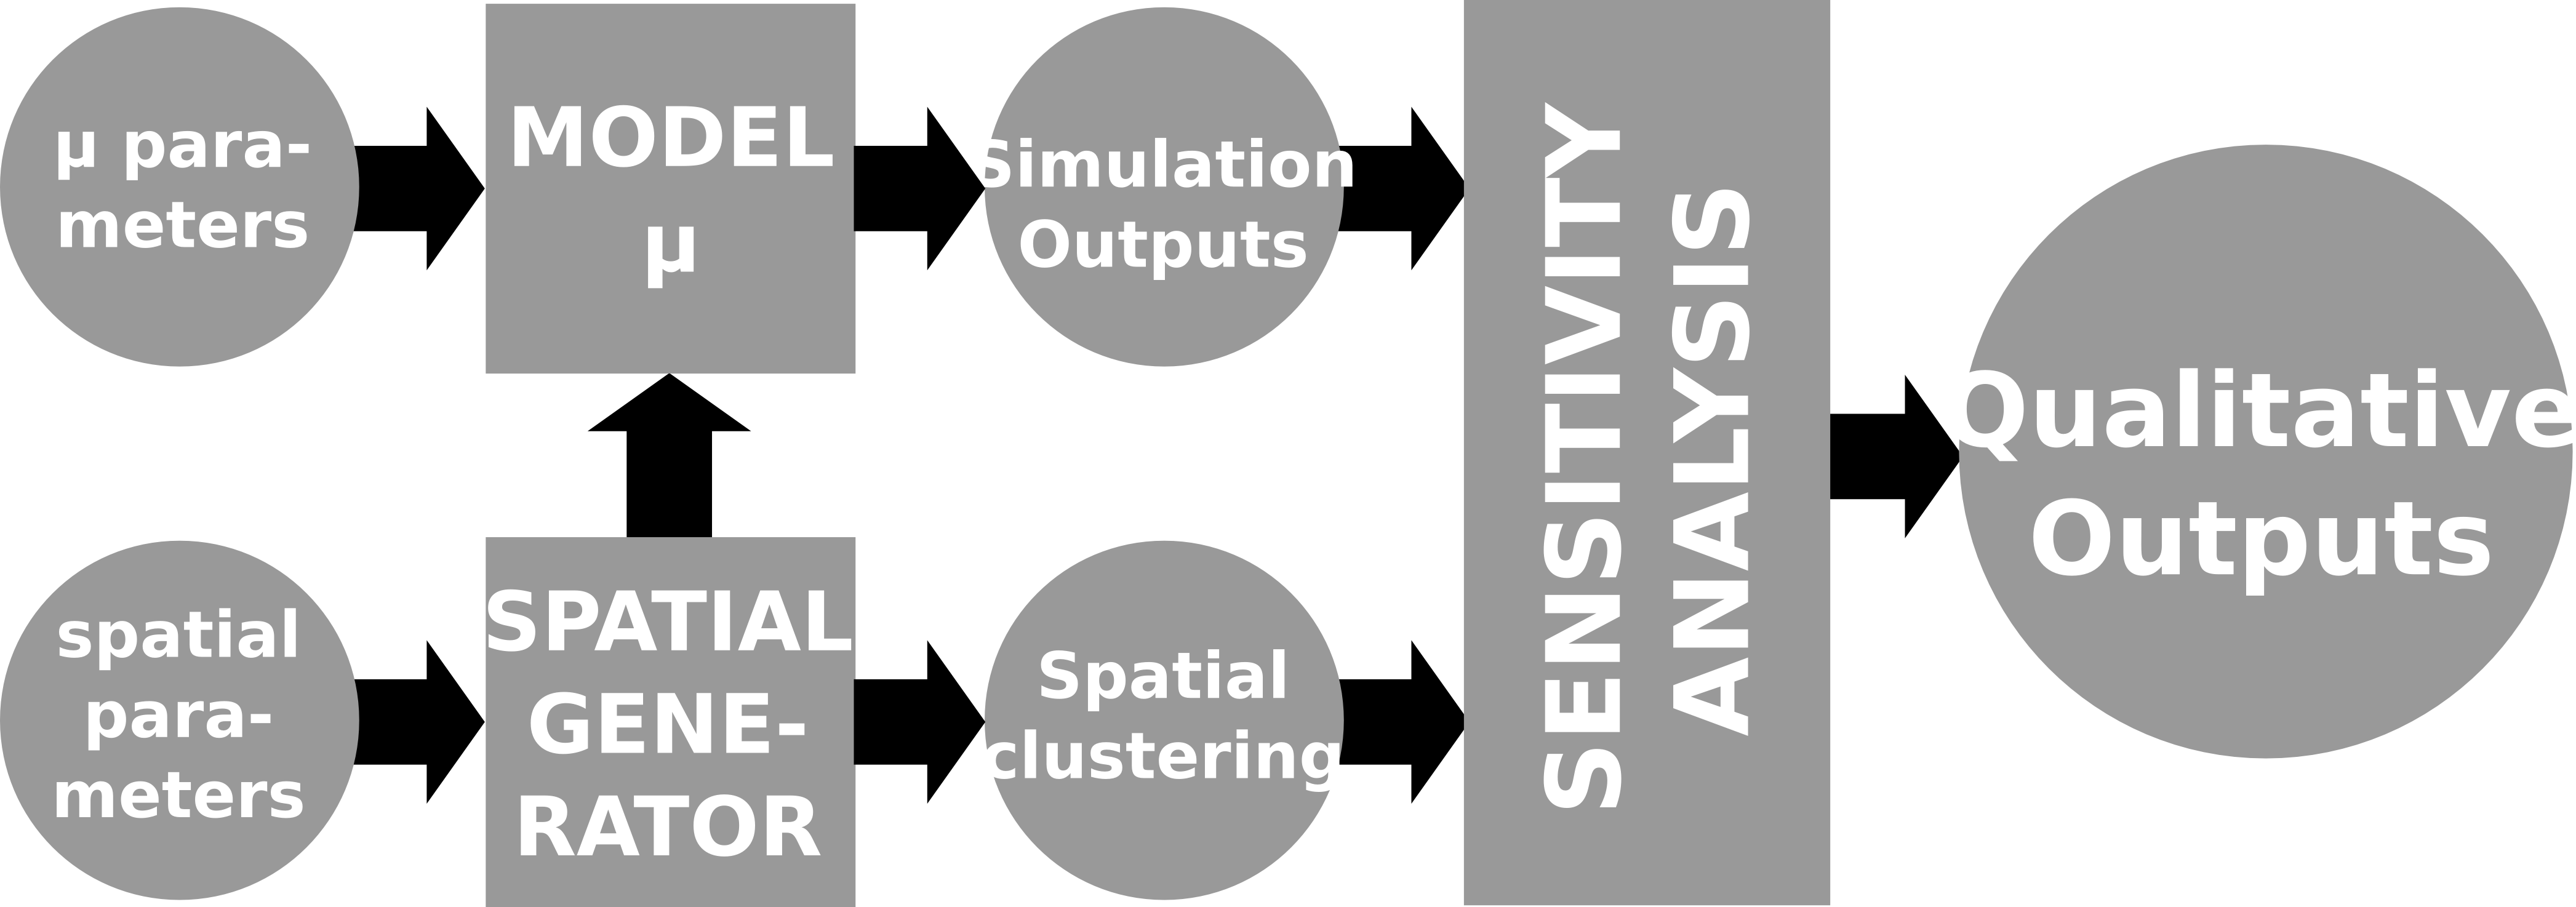
\includegraphics{figures/SchemaMeta_1.png}
} \caption{General workflow of our method} \label{fig:method} \end{center} \end{figure*} %
%%%%%%%%%%%%%%%%%%%%%%

%%%%%%%%%%%%%%%%%%%%%%
\subsection{Constructing a spatial generator}

Our spatial generator applies an urban morphogenesis model (\cite{Batty2007}), which has been generalised, explored and calibrated (\cite{Raimbault2014}). \comment[FL]{il faut que les sens de tous les paramètres soient explicités avec les équations ?} In a nutshell, grids are generated through an iterative process which adds a quantity $N$ (population) at each time step, allocating it through preferential attachment characterised by its strength of attraction $\alpha$. This first growth process is then smoothed $n$ times using a diffusion process of strength $\beta$. Grids are thus generated from the combination of the values of these four meta-parameters $\alpha$, $\beta$, $n$ and $N$, in addition to the random seed. To ease our exploration, only the distribution of density is allowed to vary rather than the size of the grid, which we fix to a 50x50 square environment of 100,000 units (cf. figure \ref{fig:spatialGen}).
\comment{A detailler en incluant les equations de morphogenese}

%%%%%%%%%%%%%%%%%%%%%%
\begin{figure*}[htbp] \begin{center} 
\resizebox{0.9\textwidth}{!}{ 
	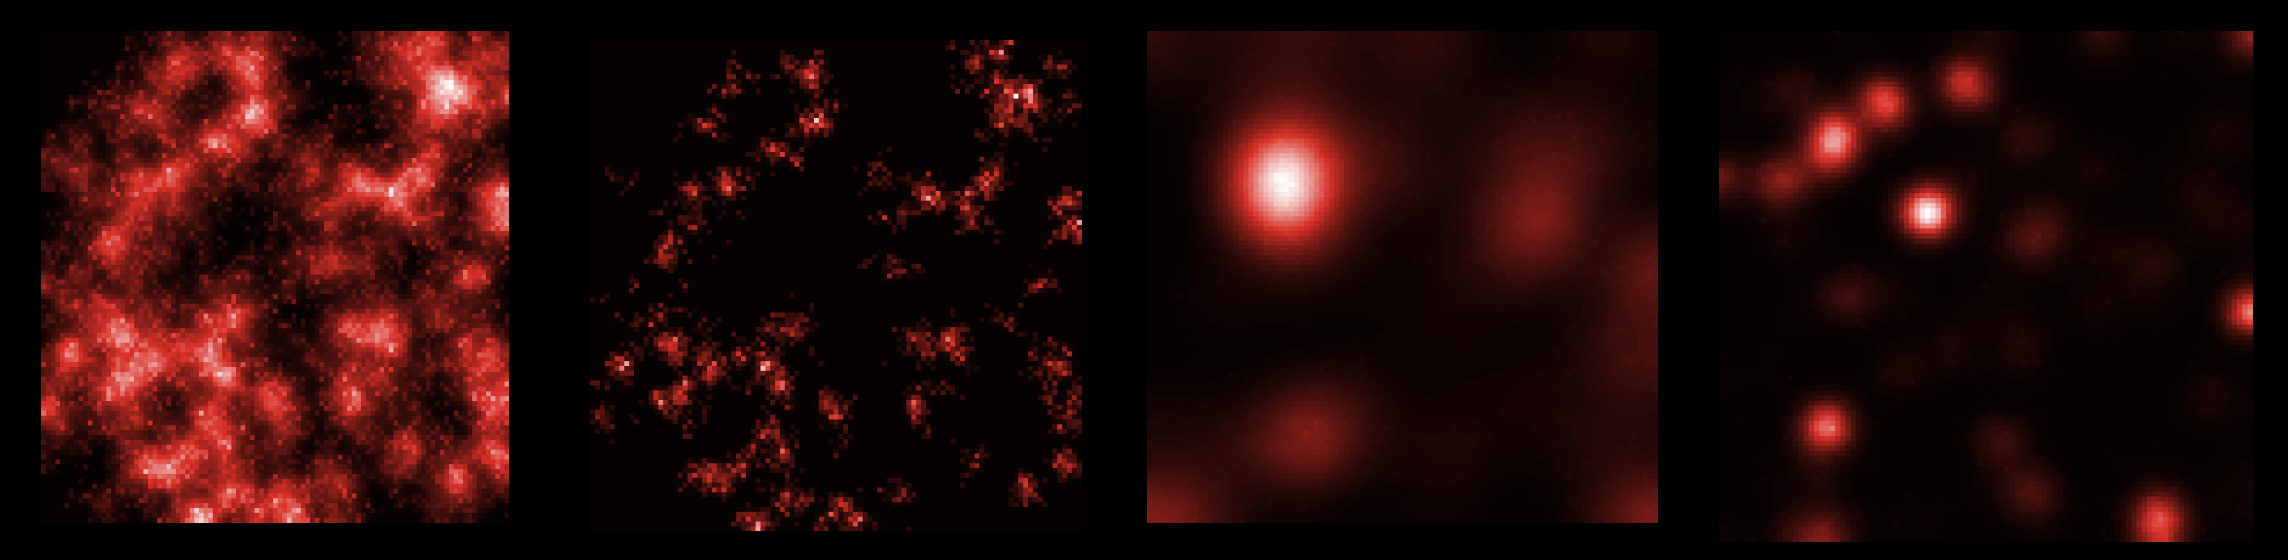
\includegraphics{figures/spatialGen.png}
} \caption{Four examples of grids produced by the spatial generator. The lighter the red, the denser the area.} \label{fig:spatialGen} \end{center} \end{figure*} %
%%%%%%%%%%%%%%%%%%%%%%


%%%%%%%%%%%%%%%%%%%%%%
\subsection{Including a (typical) variety of initial conditions in the sensitivity analysis}

In order to generate density grids which correspond to empirical density distributions, we select among the generated grids using an objective function which matches the point cloud of 110 metropolitan areas in Europe described by four dimensions: their concentration index, hierarchy index, centrality index and continuity index (cf. \cite{LeNechet2015}). A stochastic exploration of a Latin Hypercube Sampling of 2000 points in the 4-dimensional space of parameters {$\alpha$, $\beta$, $n$, $N$} gives a subset of 170 interesting grids matching empirical densities, which constituted our set of different initial spatial conditions. These are further clustered into three classes of morphology: compact (e.g. Vienna), polycentric (Liege) and discontinuous (Augsburg) in order to evaluate the non-trivial effects of urban form on simulation results. We select 15 grids of each type to work with.

%cite{Gauvinetal2009}


%%%%%%%%%%%%%%%%%%%%%%
\subsection{Comparing Phase Diagrams}

In order to test for the influence of spatial initial conditions, we need a systematic method to compare phase diagrams. Indeed, we have as many phase diagrams than we have spatial grids, what makes a qualitative visual comparison not realistic. A solution is to use systematic quantitative procedures. Several potential methods could be used \comment[MLT]{Ici je me demande si l'on ne devrait pas simplement dire que l'on a pas trouvé de méthodes de comparaisons systématiques de diagrammes de phase dans la littérature SMA ou geographic modelling, et que du coup on propose de comparer la variance intra à la variance inter-grille selon la formule ... Et je garderais la précision sur les autres méthodes que l'on aurait pu choisir pour la section de discussion}: for example in the case of the Schelling model, an anisotropic spatial segregation index (giving the number of clusters found and in which region in the parameter spaces they are roughly situated) would differentiate strong \emph{meta phase transitions} (phase transitions in the space of meta parameters). The use of metrics comparing spatial distributions, such as the Earth Movers Distance which is used for example in Computer Vision to compare probability distributions~\cite{rubner2000earth}, or the comparison of aggregated transition matrices of the dynamic associated to the potential described by each distribution, would also be potential tools. Map comparison methods, popular in environmental sciences \comment[MLT]{Et pas en géo? Qu'est-ce que ces méthodes ont de particulier?}, provide numeral tools to compare two dimensional fields~\cite{visser2006map}. To compare a spatial field evolving in time, elaborated methods such as Empirical Orthogonal Functions that isolates temporal from spatial variations, would be applicable in our case by taking time as a parameter dimension, but these have been shown to perform similarly to direct visual inspection when averaged over a crowdsourcing~\cite{10.1371/journal.pone.0178165}. To keep it simple and as such methodological considerations are auxiliary to the main purpose of this paper, we propose an intuitive measure corresponding to the share of between-diagrams variability relative to their internal variability. More formally, the distance is given by

\begin{equation}\label{eq:phase-distance}
d_r\left(\alpha_1,\alpha_2\right) = 2 \cdot \frac{d(f_{\vec{\alpha_1}},f_{\vec{\alpha_2}})^2}{Var\left[f_{\vec{\alpha_1}}\right] + Var\left[f_{\vec{\alpha_2}}\right]}
\end{equation}

where $\alpha \mapsto \left[\vec{x} \mapsto f_{\vec{\alpha}}\left(\vec{x}\right)\right]$ is the operator giving phase diagrams with $\vec{x}$ parameters and $\vec{\alpha}$ meta-parameters, and $d$ is a distance between probability distributions that can be taken for example as basic L2 distance \comment[MLT]{Euclidean? Je crois qu'il faut adapter le vocabulaire utilisé aux lecteurs d'EPB, qu'en pensez-vous?} or the Earth's Mover Distance \comment[MLT]{Si l'on mentionne les deux, ne va-t-on pas nous demander de tester l'effet du choix de l'une ou de l'autre sur nos résultats?}. For each values $\vec{\alpha_i}$, the phase diagram is seen as a random spatial field, facilitating the definition of variances and distance.
\comment[FL]{je pense que c'est un peu compliqué effectivement cette partie.}


%%%%%%%%%%%%%%%%%%%%%%
\subsection{Model Exploration Workflows as an meta-sensitivity analysis method}

The last methodological point which we need to emphasis is the relation between the workflow we introduce and model exploration workflows. The ideas of multi-modeling and extensive model exploration are nothing from new as Openshaw already advocated for ``model-crunching'' in~\cite{openshaw1983data}, but their effective use only begins to emerge thanks to the apparition of new methods and tools together with an explosion of computation capabilities. The model exploration platform OpenMole~\cite{reuillon2013openmole} allows to embed any model as a blackbox, write modulable exploration workflow using advanced methodologies such as genetic algorithms and distribute transparently the computation on large scale computation infrastructures such as clusters or computation grids. In our case, the workflow tool is a powerful way to embed both the sensitivity analysis and the meta-sensitivity analysis, and allow to couple any generator with any model in a straightforward way as soon as the model can take its spatial configuration as input or from an input file. \comment[MLT]{Je me suis permis de bouger la partie sur le multi-modeling en fin de paragraphe, mais ai essayé d'en garder l'esprit tel quel!} In this paper, we use the OpenMole platform for spatial environment and model coupling, placing ourselves in the renewed framework of multi-modeling claimed by \cite{cottineau2016back}.

%%%%%%%%%%%%%%%%%%%%%%
\section{Application cases}
%%%%%%%%%%%%%%%%%%%%%%

We use our set of initial density grids in two spatial simulation models: Schelling and Sugarscape.


%%%%%%%%%%%%%%%%%%%%%%
\subsection{Schelling's model of residential segregation}

Schelling's model consists in a abstract urban housing market where agents of different nature sense their environment, evaluate their satisfaction in terms of neighbourhood composition, and relocate if unsatisfied. It has been shown by \cite{Schelling1969} that even tolerant agents tended to produce segregated patterns because of the complexity of their local interactions. The main parameters of this model are the tolerance level (\% of agents similar to {\it ego}), the scope of sensing and the percentage of vacant spaces in the housing market. In addition, we are interested in testing the impact of the spatial distribution of housing capacity in this project, using the generated grids. \comment[MLT]{Dans le paragraphe sur Sugarscape on parle du diagramme de phase que l'on étudie en sortie, pas ici. On harmonise dans quel sens?}

%Recent attempts of running Schelling-like models beyond the chessboard grid have proved that migration decisions are not only dependent of what positions agents occupy relative to each other, but also of where they occupy these positions. \citet{FlacheHegselmann2001} show that chances for random emergence of a stable cluster of similar agents are highest in a rectangular grid and lowest in a hexagonal grid and that an irregular (Voronoi-diagram) city lattice structure favours migration stabilisation around decentralised clusters of similar agents. \citet{StaufferSolomon2007} introduce asymetric interactions and empty residences on a large and regular lattice. They reveal conjoint and non-linear effects on the vacancy rates and tolerance levels on segregation patterns. \citet{Singhetal2009} show that the segregation patterns obtained by Schelling for certain tolerance values are strictly a small city phenomenon (8x8 city-lattice) and do not work for a larger spatial lattice (100x100), where segregation appears only for certain combinaisons of tolerance threshold and vacancy density values. \citet{Gauvinetal2010} run Schelling's segregation process in an open city-lattice to study how the variations in tolerance levels, vacancy rates and city attractiveness may create lines of vacancy lots between clusters of agents. They conclude on the functional role of vacancies, which allow weakly tolerant agents to live and be satisfied in a city environment they nevertheless perceive as hostile. \citet{Banos2012} compares the behaviour of Schelling segregation model on city lattices formalized as either grid, random, scale-free and Sierpinski networks and concludes that the presence of cliques in graph-based urban structures favor segregationist behaviours. Interestingly, \citet{HatnaBenenson2012} show that their model replications run on a 50x50 torus with 2\% of empty cells were not sensitive to the initial patterns (random and fully segregated distribution of agents). In this paper, we build on the contributions of these previous studies and go further by systematically measuring the impact of the city lattice on Schelling model behaviour so far only assessed through a small set of illustrative spatial structures. \comment[MLT]{Le remettre en moins détaillé dans l'intro en lien avec les catégories de prise en compte de la forme de la grille.}


%%%%%%%%%%%%%%%%%%%%%%
\subsection{Sugarscape model of resource extraction and population settlement}

Sugarscape is a model of resource extraction which simulates the unequal distribution of wealth within a heterogenous population (\cite{EpsteinAxtell1996}). Agents of different vision scopes and different metabolisms harvest a self-regenerating resource available heterogeneously in the initial landscape, they settle and collect this resource, which leads some of them to survive and others to perish. The main parameters of this model are the number of agents, their minimal and maximal resource. In addition, we are interested in testing the impact of the spatial distribution of the resource in this project, using the generated grids. The outcome of the model is measured as a phase diagram of an index of inequality for ressource distribution (Gini index). We extend the implementation with agents wealth distribution of~\cite{li2009netlogo}.


%%%%%%%%%%%%%%%%%%%%%%
\section{Results}
%%%%%%%%%%%%%%%%%%%%%%

\comment[FL]{il faudrait peut être davantage renforcer l'analyse a propos de figure 1 de si c'est plutôt les mu parameters ou les spatial parameters qui ont une grosse influence sur les résultats.}



%%%%%%%%%%%%%%%%%%%%%%
\subsection{Schelling's model}

We proceed to 4,500,000 simulation runs of the Schelling model (1000 parameter combinations x 45 density grids x 100 replications), using OpenMOLE to distribute the computation, and apply segregation measures to characterise the results. We find that the different urban morphologies impact the parameter interaction patterns, and that polycentric and discontinuous cities appear systematically more segregated than compact cities in terms of dissimilarity and entropy index.



%%%%%%%%%%%%%%%%%%%%%%
\subsection{Sugarscape model}

For Sugarscape, 2,500,000 simulations (1000 parameter points x 50 density grids x 50 replications) allow us to show that the model is more sensitive to space than to its other parameters, both qualitatively and quantitatively: the amplitude of variations across density grids is larger than the amplitude in each phase diagram, and the behavior of phase diagram is qualitatively different in different regions of the morphological space.

More precisely, we explore a grid of a basic parameter space of the model, which three dimensions are the population of agents $P\in \left[10;510\right]$, the minimal initial agent ressource $s_{-}\in \left[10;100\right]$ and the maximal initial agent ressource $s_{+}\in \left[110;200\right]$. Each parameter is binned into 10 values, giving 1000 parameter points. We run 50 repetitions for each configuration, what yield reasonable convergence properties. The initial spatial configuration varies across 50 different grids, generated by sampling meta-parameters for the generator in a LHS. We did not use the clustered grids to test the flexibility of our framework, which is demonstrated in this case by a direct sequential coupling of the generator and the model. We mesure the distance of all 3-dimensional phase diagrams to the reference phase diagram computed on the default model setup (see Fig.~\ref{fig:sugarscape-distance} for its morphological positioning regarded generated grids), using equation~\ref{eq:phase-distance} with the L2 distance to ensure direct interpretability. Indeed, it gives in that case the average squared distance between corresponding points of the phase diagrams, relative to the average of the variance of each. Therefore, values greater than 1 will mean that inter-diagram variability is more important than intra-diagram variability.

% summary stats
%   Min. 1st Qu.  Median    Mean 3rd Qu.    Max. 
% 0.08909 0.19790 1.52200 1.29600 2.16400 2.98100 

We obtain a very strong sensitivity to initial conditions, as the distribution of the relative distance to reference across grids ranges from 0.09 to 2.98 with a median of 1.52 and an average of 1.30. It means that in average, the model is more sensitive to meta-parameters than to parameters, and the relation variation can reach a factor of 3. We plot in Fig.~\ref{fig:sugarscape-distance} their distribution in a morphological space. The reduced morphological space is obtained by computing 4 raw indicators of urban form, namely Moran index, average distance, rank-size slope and entropy (see~\cite{LeNechet2015} for precise definition and contextualization), and by reducing the dimension with a principal component analysis for which we keep the first two components (92\% of cumulated variance). The first measures a ``level of sprawl'' and of scattering, whereas the second measures aggregation.\footnote{We have $PC1 = 0.76\cdot distance + 0.60\cdot entropy + 0.03\cdot moran + 0.24\cdot slope$ and $PC2 = -0.26\cdot distance + 0.18\cdot entropy + 0.91\cdot moran + 0.26\cdot slope$.} We find that grids producing the highest deviations are the ones with a low level of sprawl and a high aggregation. It is confirmed by the behavior as a function of meta-parameters, as high values of $\alpha$ also yield high distance. In terms of model processes, it shows that congestion mechanisms induce rapidly higher levels of inequality.


% pca of morphological space
% "","PC1","PC2","PC3","PC4"
%"distance",0.762358566609464,-0.260991693298744,0.200656405132039,0.557162237616392
%"entropy",0.601306167355116,0.181706245959277,0.0958379422351422,-0.772158547261002
%"moran",0.0311129390452153,0.912155429075071,0.30114271129527,0.276256268103684
%"slope",0.237217819823539,0.258531718397015,-0.927289147645628,0.130475642169329

%%%%%%%%%%%%%
\begin{figure}
\centering
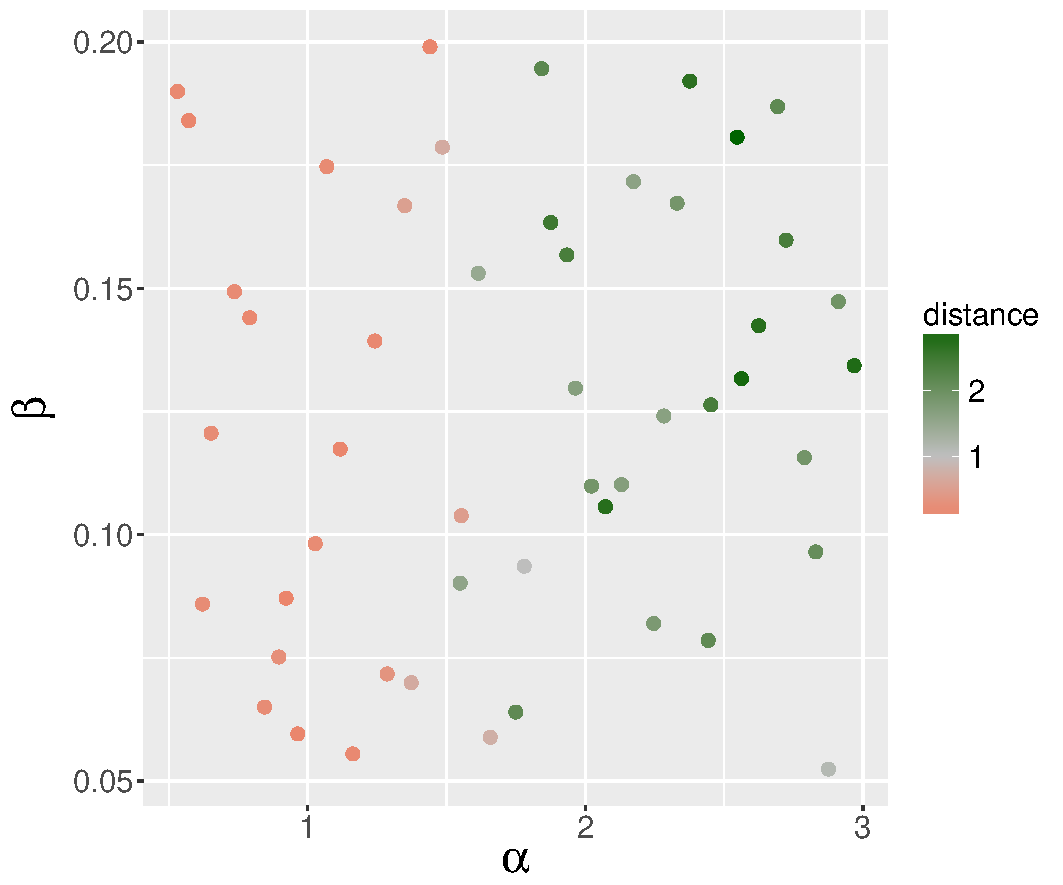
\includegraphics[width=0.5\textwidth]{figures/relativedistance_metaparams}\\
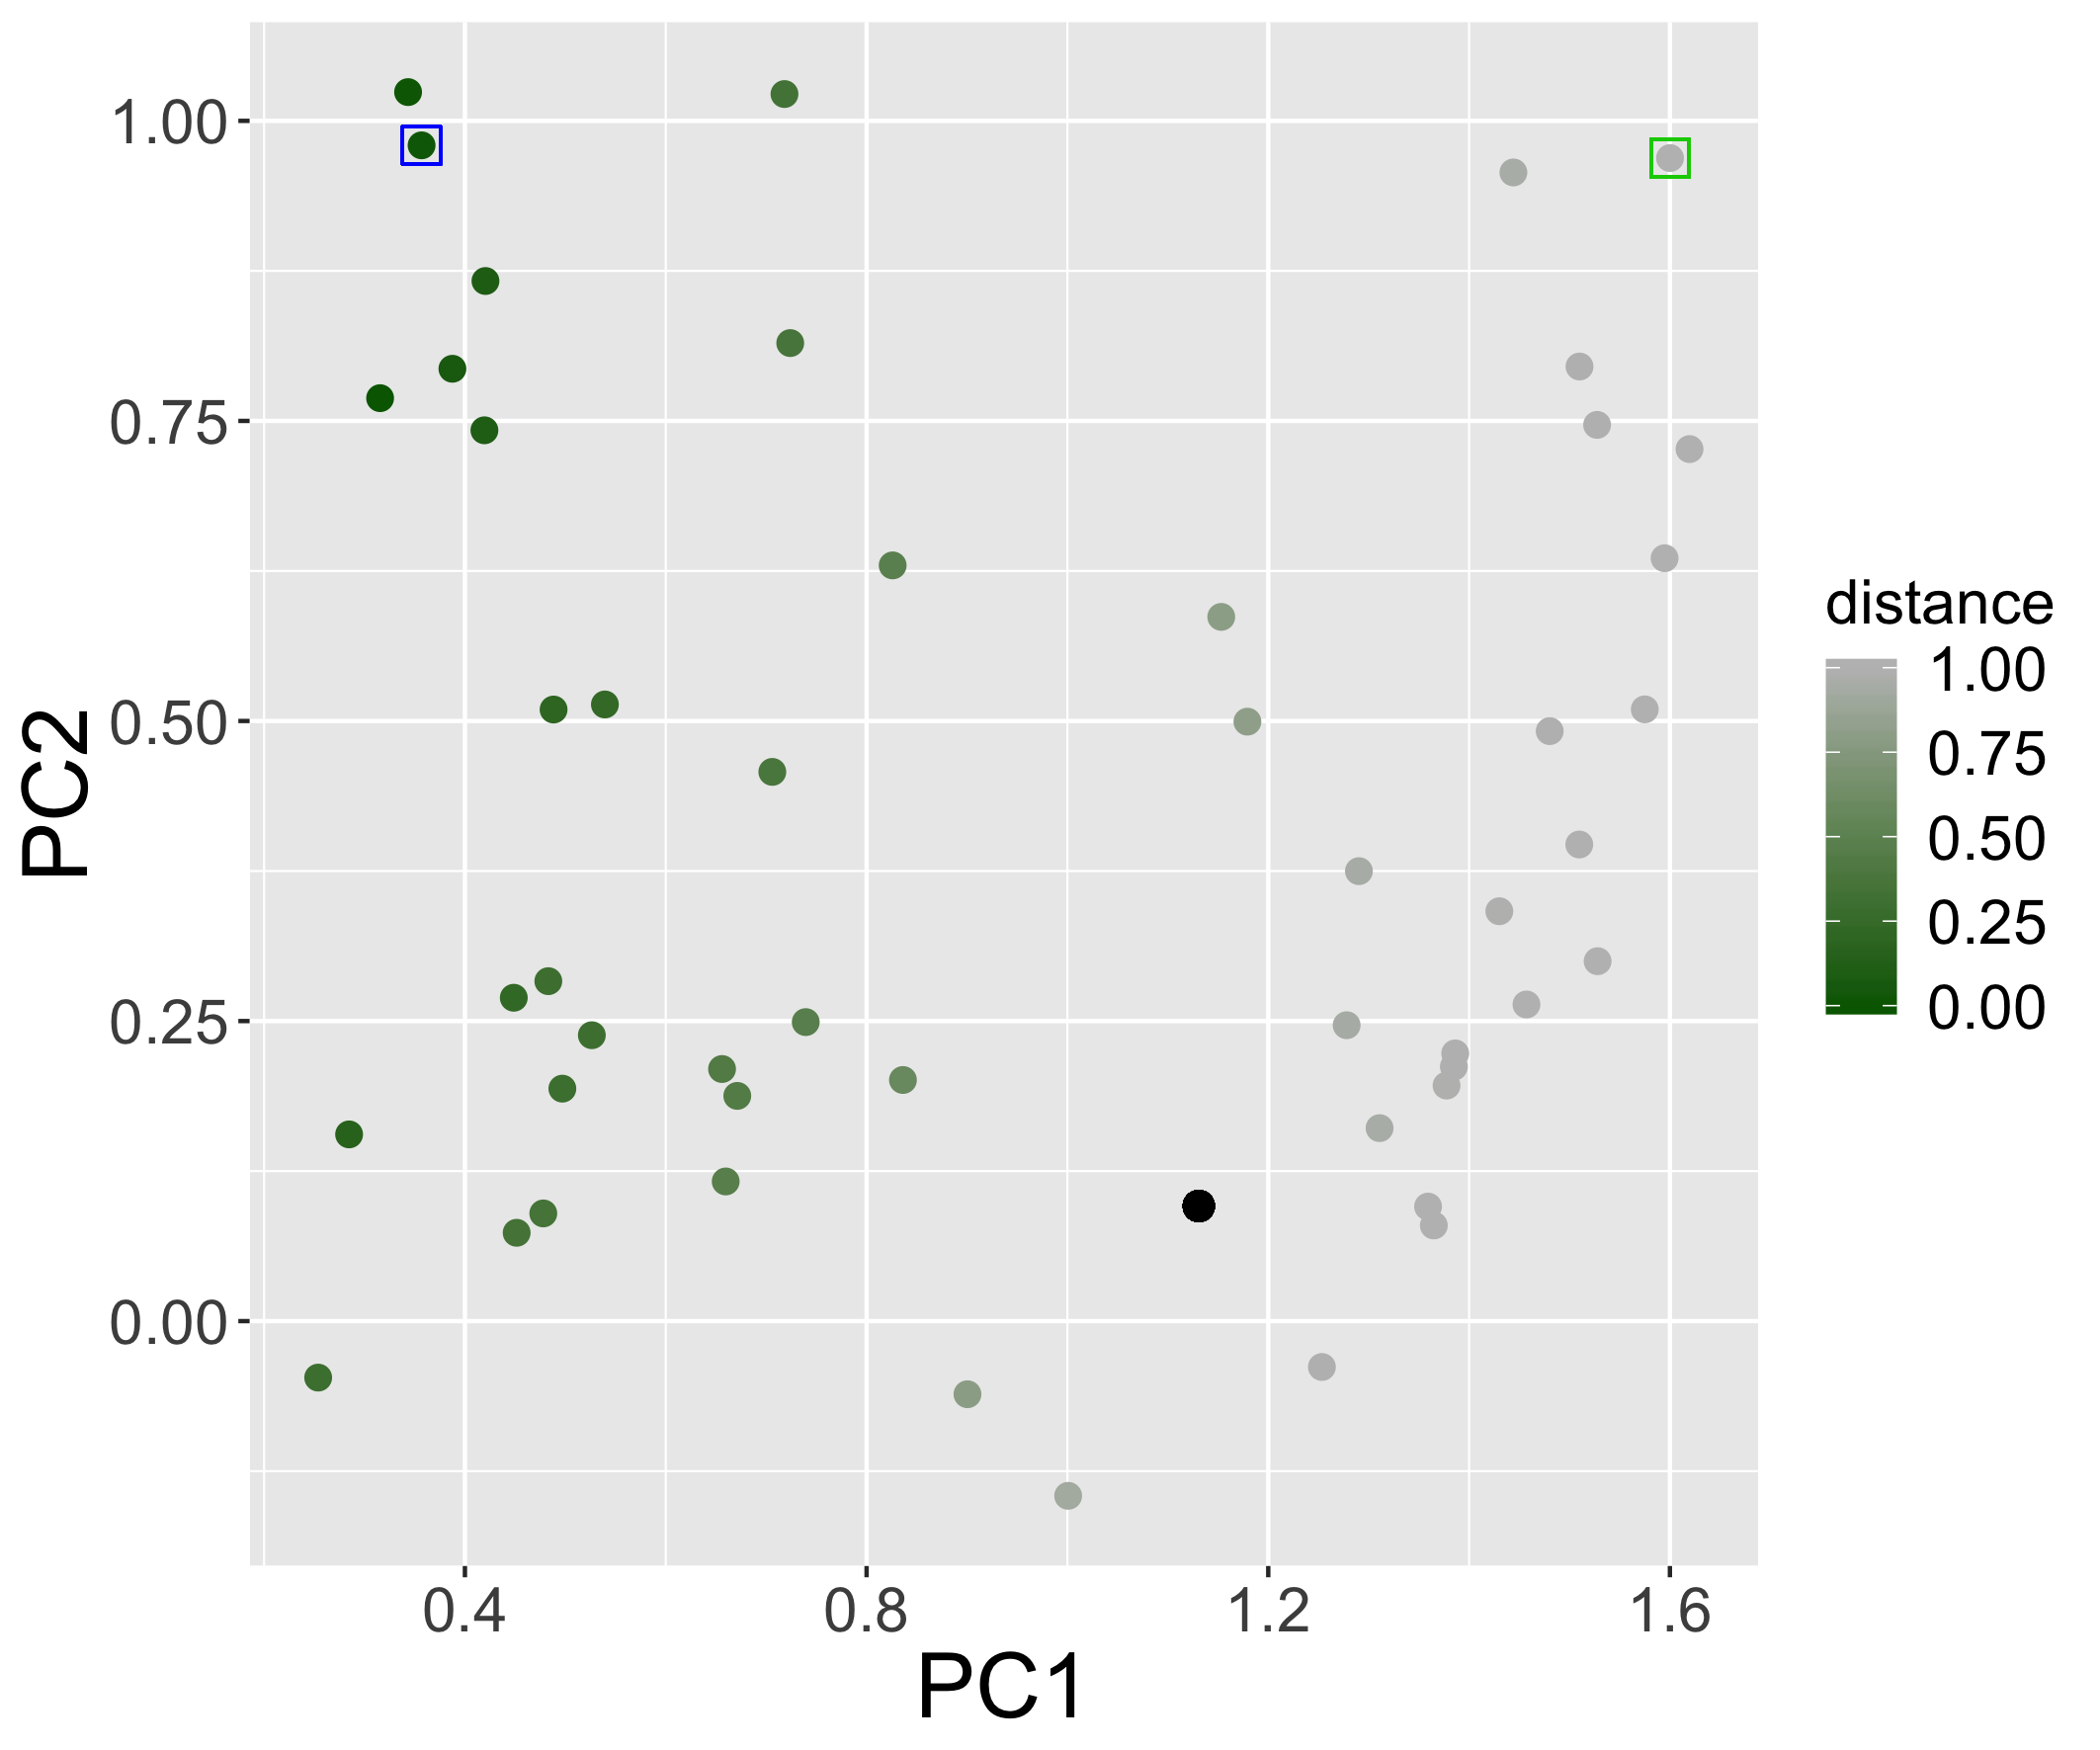
\includegraphics[width=0.5\textwidth]{figures/relativedistance_morphspace}
\caption{\textbf{Relative distances of phase diagrams to the reference across grids.} (Top) Relative distance as a function of meta-parameters $\alpha$ (strength of preferential attachment) and diffusion ($\beta$, strength of diffusion process). (Bottom) Relative distance as a function of two first principal components of the morphological space (see text). Red point correspond to the reference spatial configuration. Green frame and blue frame give respectively the first and second particular phase diagrams shown in Fig.~\ref{fig:sugarscape-phasediagrams}.}
\label{fig:sugarscape-distance}
\end{figure}
%%%%%%%%%%%%%



% phase diagrams -> ok well different qualitatively
%          spAlpha spDiffsteps spDiffusion spGrowth spPopulation
% id=27 : 0.7913103    2.376837   0.1440293 157.4147 4852.746
% id=0 : 2.562398    3.753032   0.1316788 128.4632 4753.983
% maxSugar = 110


%%%%%%%%%%%%%
\begin{figure}
\centering
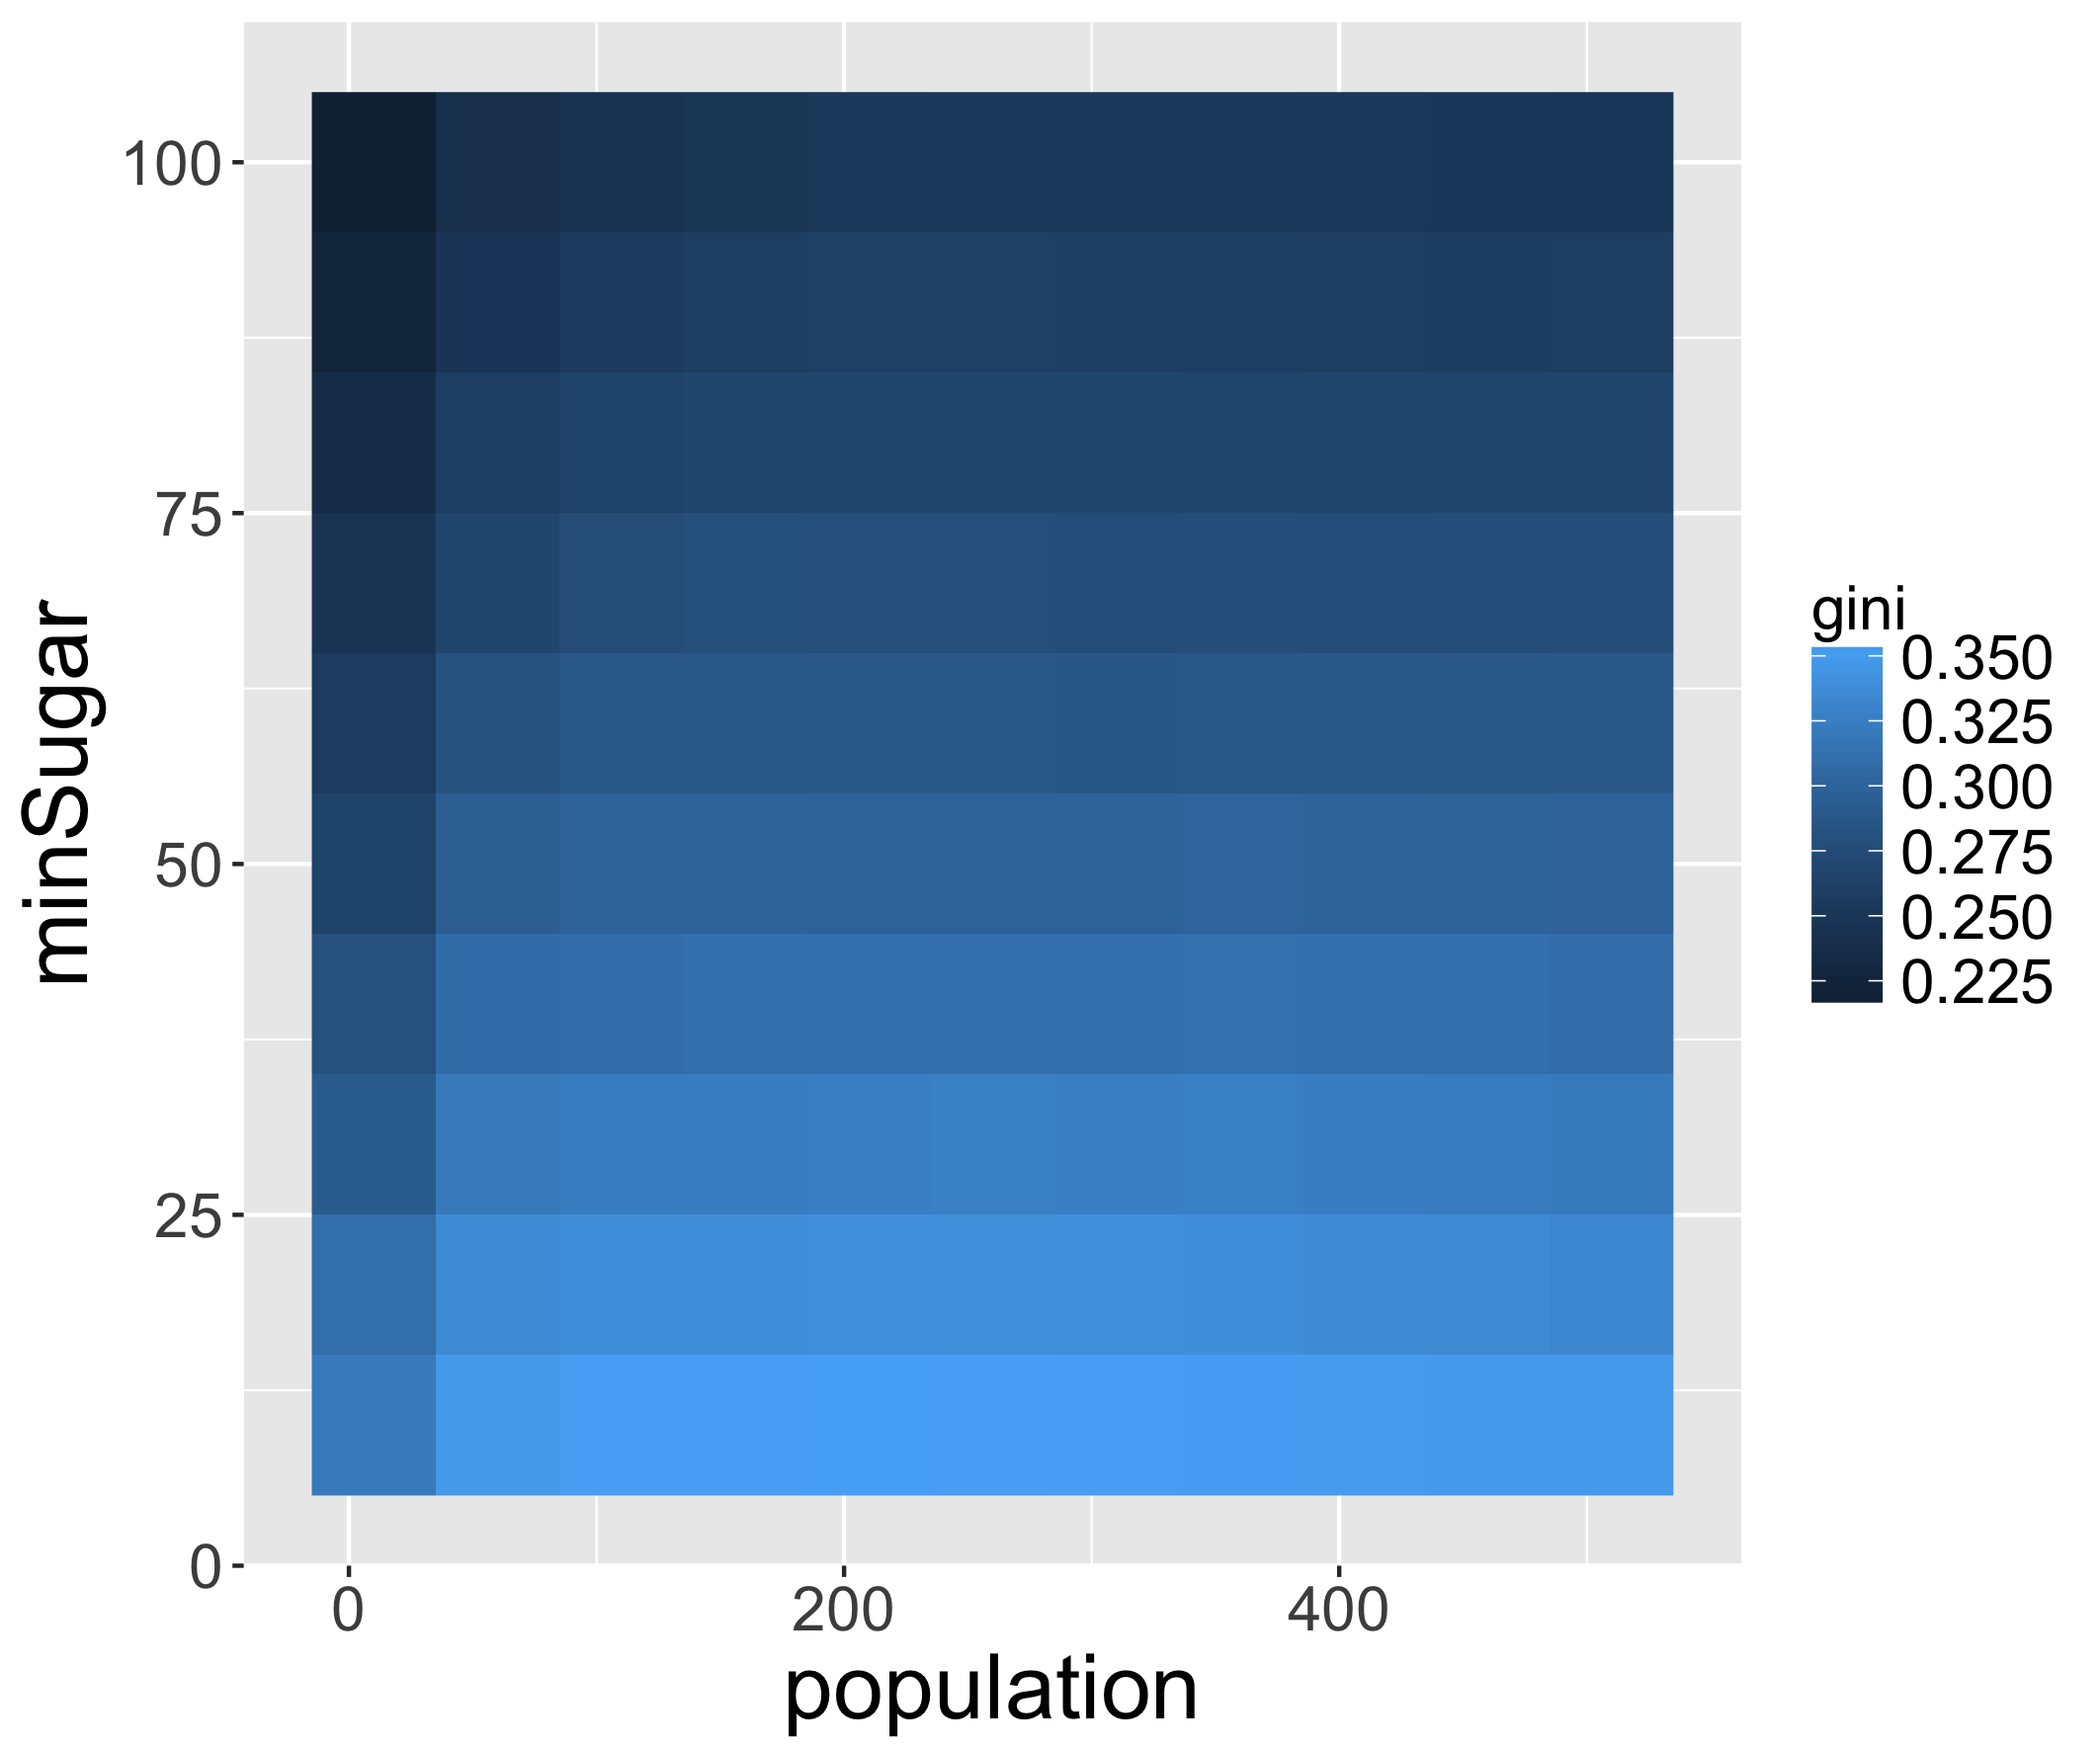
\includegraphics[width=0.24\textwidth]{figures/phasediagram_id27_maxSugar110}
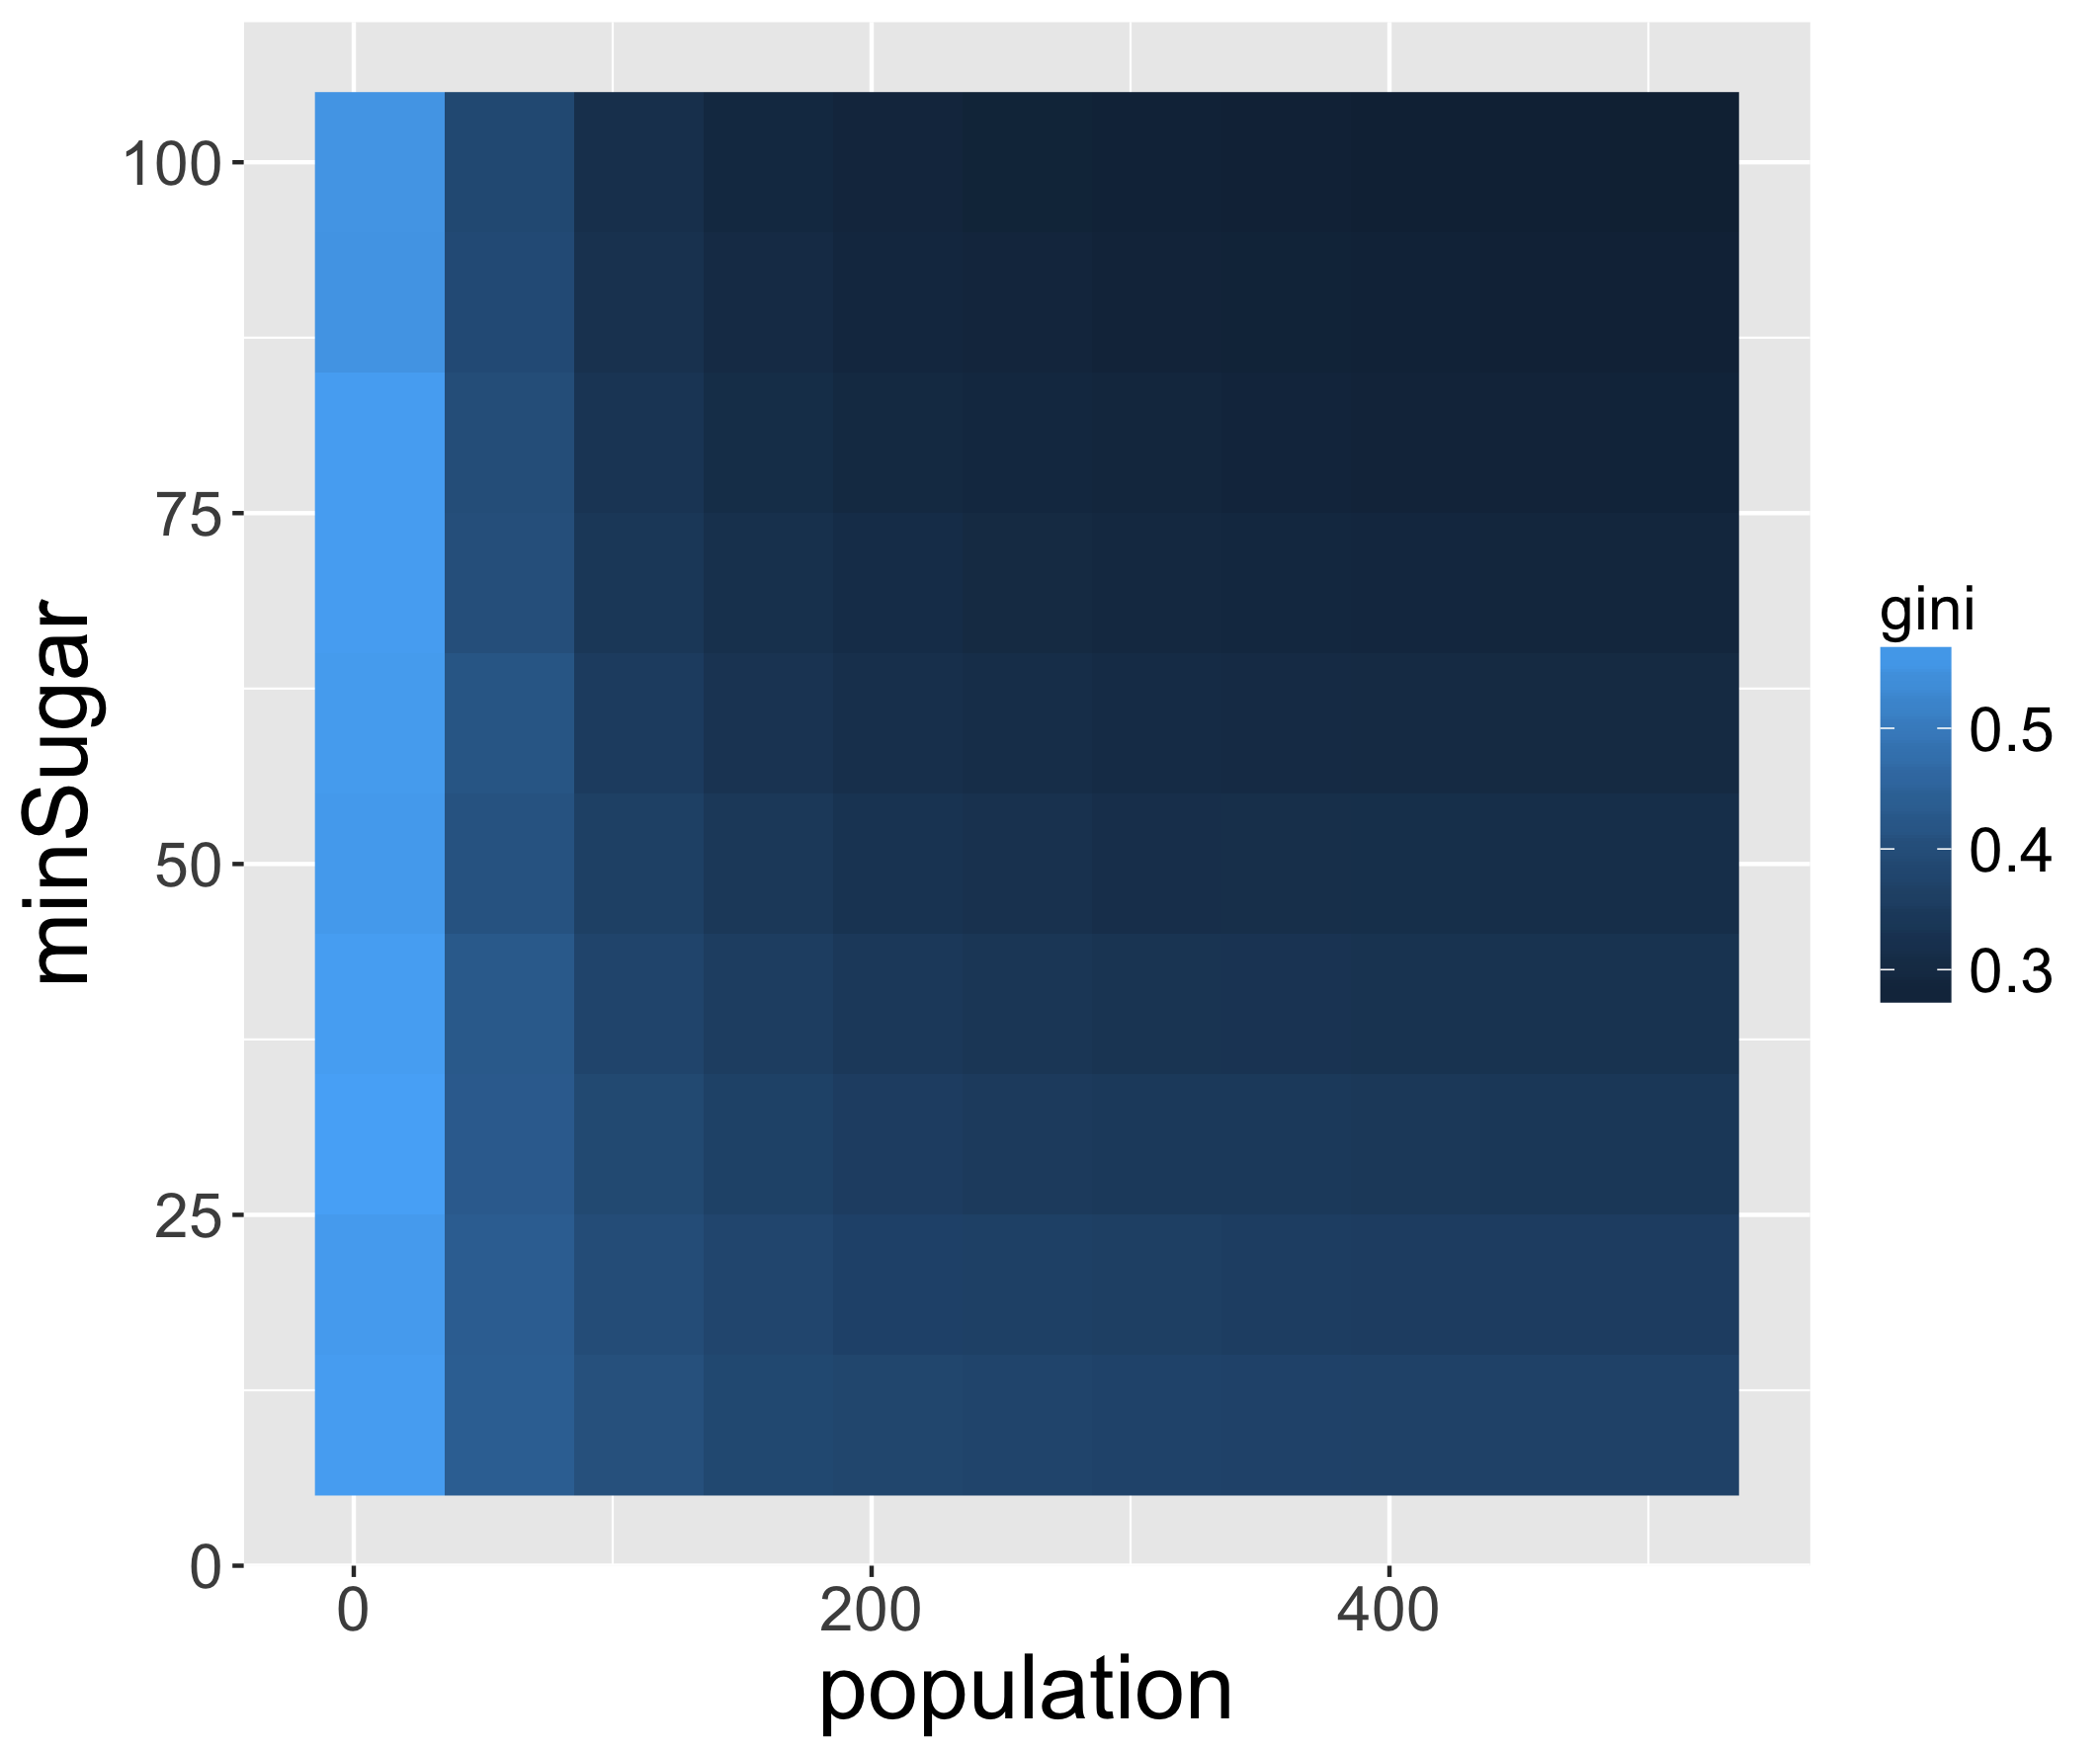
\includegraphics[width=0.24\textwidth]{figures/phasediagram_id0_maxSugar110}
\caption{\textbf{Examples of phase diagrams.} We show two dimensional phase diagrams on $(P,s_-)$, both at fixed $s_+ = 110$. (Left) Green frame, obtained with $\alpha = 0.79$, $n=2$, $\beta = 0.14$, $N=157$; (Right) Blue frame, obtained with $\alpha = 2.56$, $n=3$, $\beta = 0.13$, $N=128$.}
\label{fig:sugarscape-phasediagrams}
\end{figure}
%%%%%%%%%%%%%

We now check the sensitivity in terms of qualitative behavior of phase diagrams. We show the phase diagrams for two very opposite morphologies in term of sprawling, but controlling for aggregation with the same $PC2$ value. These correspond to the green and blue frames in Fig.~\ref{fig:sugarscape-distance}. The behaviors are rather stable for varying $s_+$, what means that the poorest agents have a determinant role in trajectories. The two examples have not only a very distant baseline inequality (the ceil of the first 0.35 is roughly the floor of the second 0.3), but their qualitative behavior is also radically opposite: the sprawled configuration gives inequalities decreasing as population decreases and decreasing as minimal wealth increases, whereas the concentrated one gives inequalities strongly increasing as population decreases and also decreasing with minimal weights but significantly only for large population values. The process is thus completely inverted, what would have significant impacts if one tried to schematize policies from this model. This second example confirms thus the importance of sensitivity of simulation models to the initial spatial conditions.

%%%%%%%%%%%%%%%%%%%%%%
\section{Discussion}
%%%%%%%%%%%%%%%%%%%%%%

\comment{NetLogo qui influence la formalisation de l'espace dans les modèles alors que formalisation de ce dernier peut être plus poussée dans la description du modèle original.}

% \hfill \break
% \itshape{This is a sub, subheading}\normalfont

% \hfill\break

%
%
%\begin{table}[htp]
%
%\begin{center}
%\begin{tabular}{c c c c}
%\arrayrulecolor{black}
%\hline 
%This & Is & A & Table\\
%\arrayrulecolor{lightgray}
%\hline 
%\arrayrulecolor{black}
%Label & 0.1 & 0.2 & 0.3\\
%Label & 1.0 & 2.0 & 3.0\\
%\hline
%\end{tabular}
%\end{center}
%\label{first_table}
%\caption{This is a table caption}
%\end{table}%
%
%
%
%\begin{equation}
%a^2 + b^2 = c^2
%\tag*{Equation 1}
%\end{equation}

%%%%%%%%%%%%%
% Acknowledgements

\begin{acks}
The authors acknowledge the funding of their institutions and the EPSRC project number EP/M023583/1. Results obtained in this paper were computed on the vo.complex-system.eu virtual organization of the European Grid Infrastructure ( http://www.egi.eu ). We thank the European Grid Infrastructure and its supporting National Grid Initiatives (France-Grilles in particular) for providing the technical support and infrastructure.
\end{acks}




%%%%%%%%%%%%
%% References
%%%%%%%%%%%%


\bibliographystyle{SageH}
\bibliography{spacematters,biblio}


\end{document}
